\documentclass[1p]{elsarticle}

\usepackage{lineno,hyperref}
\modulolinenumbers[5]
\usepackage[utf8]{inputenc}
\usepackage[spanish]{babel}
\usepackage{amsmath}
\usepackage{todonotes}
\usepackage{listings}
\usepackage{graphicx}
\usepackage{amsfonts}
\usepackage{wrapfig}
\usepackage[toc,page]{appendix}
\usepackage{amssymb}
\newtheorem{thm}{Teorema}
\newtheorem{lem}[thm]{Lema}
\newdefinition{rmk}{Remark}
\newproof{pf}{Demostración}
\newproof{pot}{Demostración del Teorema \ref{thm2}}
 \graphicspath{ {./images/} }
 \usepackage{listings}
 \usepackage{color}
 
 \definecolor{codegreen}{rgb}{0,0.6,0}
 \definecolor{codegray}{rgb}{0.5,0.5,0.5}
 \definecolor{codepurple}{rgb}{0.58,0,0.82}
 \definecolor{backcolour}{rgb}{0.95,0.95,0.92}
 
 \lstdefinestyle{mystyle}{
 	backgroundcolor=\color{backcolour},   
 	commentstyle=\color{codegreen},
 	keywordstyle=\color{magenta},
 	numberstyle=\tiny\color{white},
 	stringstyle=\color{codepurple},
 	basicstyle=\footnotesize,
 	breakatwhitespace=false,         
 	breaklines=true,                 
 	captionpos=b,                    
 	keepspaces=true,                 
 	numbers=left,                    
 	numbersep=5pt,                  
 	showspaces=false,                
 	showstringspaces=false,
 	showtabs=false,                  
 	tabsize=2
 }
 
 \lstset{style=mystyle}
%%\bibliographystyle{IEEEannot}

%% `Elsevier LaTeX' style
\bibliographystyle{elsarticle-num}
%%%%%%%%%%%%%%%%%%%%%%%
\usepackage{setspace}  
\begin{document}

\begin{frontmatter}

\title{State of art in the Quantum Physics' explanation of the animals' magnetic sense }

%% Group authors per affiliation:
\author{Bartolomé Ortiz Viso}
\address{Master en Física y Matemáticas\\ Universidad de Granada\\23/06/2018}

\begin{abstract}
This work offers a brief look in the quantum physics' explanation of the animals' magnetics sense. It is based on the talks given by Thorsten Ritz in BIOMAT2018 congress, whose main topic was quantum biology. The aim of these pages is to explain the main results in this particular topic (magnetic sensing), its connections with quantum physics and also to offer some other highlights of the talks. Moreover the reader can find some personal opinions and possibles advances that I discussed with Thorsten himself. 
\end{abstract}

\begin{keyword}
 \texttt{Quantum Physics} \sep \texttt{Mathematics}\sep \texttt{Quantum Biology} \sep \texttt{Magnetic Sensing}
\end{keyword}

\end{frontmatter}
\setlength\parindent{0pt}
\linenumbers


\section{Background biológico}
\spacing{1.5}

Nos encontramos ante un delicado campo de estudio. En esta primera sección vamos a exponer los principales hallazgos en cuanto a el conocimiento de que diversas especies animales poseen la capacidad de sentir campos magnéticos, en particular el campo magnético terrestre.

Destacamos que aun hoy sabemos bastante poco sobre este sentido. Si bien los mecanismos hoy día están investigándose, estamos lejos de comprender este sentido completamente. Factores como los mecanismos fisicos implicados, las moleculas receptoras, la transducción de la señal o el procesado neuronal de la misma, son aun objetivo d intenso debate y estudio.

Aun asi, aunque no sepamos todos los mecanismos involucrados, conocemos la existencia y algunos de los límites de este sentido, gracias a los experimentos que se llevan a cabo con diferentes especies animales. Son las respuesta comportamentales que se observan en los sujetos de los experimentos, las que nos presentan el mayor indicio de que este sentido existe y tiene un alto impacto en su dinámica, aun sin saber como funciona exactamente.

En primer lugar, en estos estudios es habitual comprender la tierra como un barra magnética gigante (gigante no nos debe conducir a error: el campo magnético terrestre es difícil de detectar biológicamente). Y, nos interesamos por campo magnético vectorial. Aunque en cada punto podemos encontrar 2 componentes : horizontal y vertical, solemos medir la componente horizontal, y también es destacable el ángulo de inclinación, como veremos durante los experimentos. 

Uno de los animales más habituales en este tipo de experimentos son los pájaros. Es de sobra conocido que muchas aves tienen pautas de migración muy interesantes y complejas, en las que tener sensibilidad al campo magnético terrestre juega un papel crucial.

 En este área los primeros experimentos fueron gracias al desarrollo de instrumental experimental especifico, puesto que los métodos observacionales se mostraron ineficaces. Como se puede leer en \cite{embudo}, los investigadores desarrollaron un embudo \ref{embudo_1} para percibir la dirección que toman los pájaros durante los experimentos. 
  \begin{figure}
  	\centering
  	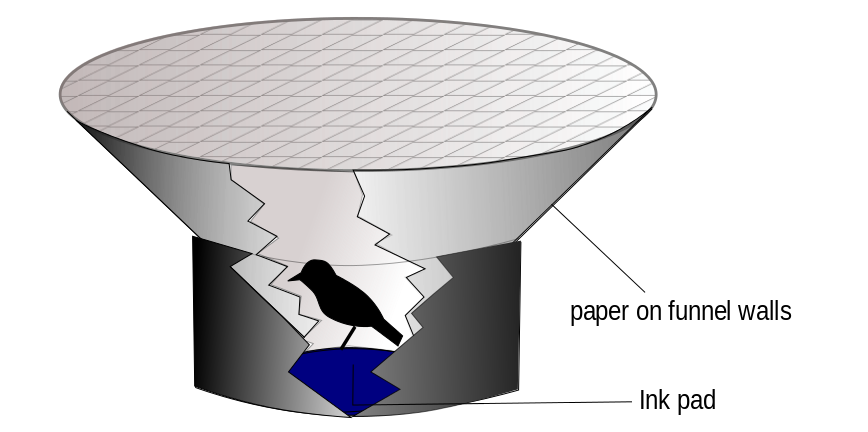
\includegraphics[width=0.5\textwidth]{emlen_funnel}
  	\caption{Diagrama de embudo de Emlen}
  	\label{embudo_1}
  \end{figure}
  
 Uno de los primeros estudios con esta técnica centrado en el campo magnético terrestre fue llevado a cabo en 1972 \cite{petirrojo}. En el se escogió al petirrojo europeo (\textit{Erithacus rubecula}),el cual está distribuido por toda Europa, principalmente en la región meridional y occidental del continente, donde habita todo el año, siendo migrante parcial en el norte de Europa y noroeste de África.
Se recogieron varios de estos individuos y, una vez dentro de un embudo de Emlen, se procedió a cambiar artificialmente el campo magnético. Se pudieron obtener algunas comclusiones: 
\begin{itemize}
	\item Los pájaros siguieron el norte, tanto en el grupo de control como cuando el norte era alterado artificialmente.\ref{embudo_2}
	\item Los pájaros eran capaces de detectar la inclinación, pero no la polaridad, por lo que la componente vertical es importante.
\end{itemize}
\begin{figure}
	\centering
	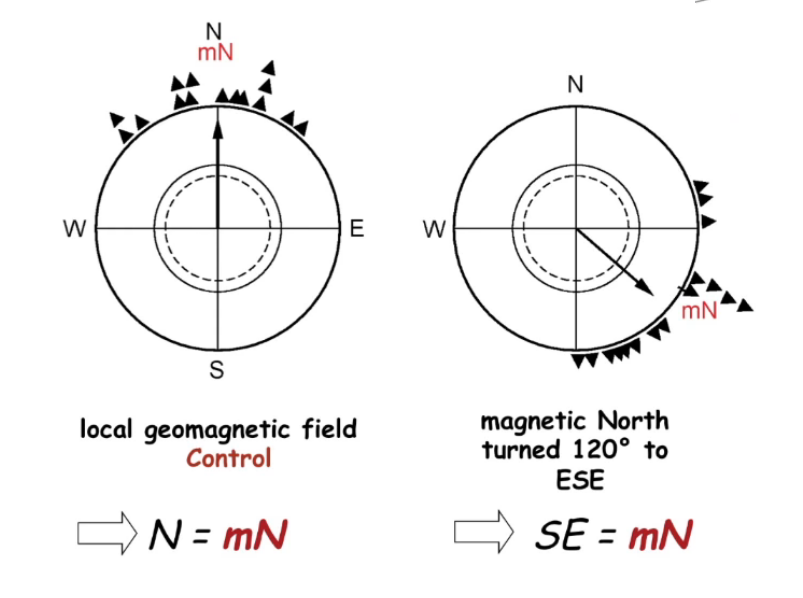
\includegraphics[width=0.7\textwidth]{embudopollos}
	\caption{Resultados del cambio en el campo magnetico}
	\label{embudo_2}
\end{figure}

Se compuso así la primera prueba de la sensibilidad magnetica de estos animales. Más tarde fueron incluidos multitud de experimentos relacionados con esta capacidad, los cuales voy a nombrar brevemente para finalizar esta parte.

\begin{itemize}
	\item Se ha observado ciertas relaciones entre la luz y la cantidad de la misma. Aunque no hay una correlacion obvia entre fotoreceptores y comportamiento, sin embargo, la manipulacion con el ciclo regulatorio puede ser la causa. Volveremos sobre este tema durante las evidencia de la importancia de este 
	\item Se ha observado que tapar el ojo derecho produce desorientación, mientras que tapar el ojo izquierdo no, con lo que se plantea la posibilidad de que la "brujula" se encuentre en este ojo.
	\item Se han encontrado evidencias de que los pajaros pueden resetear su percepcion en ciclos de un día. Estudios mostraban que pajaros que tenían una dirección equivocada de manera artificial, corregían su rumbo cuando pasaba un día.
\end{itemize}

Por último, estudios de comportamientos se han llevado a cabo en muchos otros animales, de los cuales, destacamos: 
\begin{itemize}
	\item Gallina común: En este caso el estudio presenta una clara muestra de condicionamiento magnético
	\item Tortuga boba: este animal ofrece unos comportamientos migratorios fascinantes. En experimentos llevados a cabo en piscinas, se pudo observar esa percepcion al campo magnetico como la mostrada en pájaros.
	\item Las moscas de la fruta tambien presentan este tipo de comportamiento
	\item Muchos otros animales: invertebrados, mamiferos, peces, etc.
\end{itemize}

Hasta la fecha no se ha encontrado evidencia alguna de que los seres humanos poseamos esta capacidad.

Una vez que tenemos una visión global de este fenómeno, vamos a adentrarnos en los mecanismos que pueden motivarlo.


\section{Mecanismo de par radical}
\spacing{1.5}
Es usual encontrar dos vertientes principales sobre los mecanismos implicados en la magnetorecepcion de los animales.
Por un lado tenemos las particulas de oxido de hierro, sin embargo, estas no tienes ninguna implicacion relacionada con la mecánica cuántica con lo que durante las charlas nos centramos en la vertiente que si tienes estas implicaciones: el mecanismo de radical par.

Durante los años 70 se descubre que campos magneticos débiles puden afectar a las reacciones quimicas, usando luz para  foto-inducir una transferencia de electrones, dando lugar a un par de moleculas con un par de electrones separados pero entrelzados entre sí.

Ahora bien, los electrones tienen la propiedad del spin: todos los electrones giran en un sentido alrededor de su eje. Este giro genera un campo magnético. Como se puede intuir, el spin puede encontrarse en dos estados, que habitualmente estan relacionados mediante el concepto de enlazamiento cuantico. Sin embargo, al separarse pueden darse dos estados: \textit{triplet} (cuando van en el mismo sentido) y \textit{singlet} (cuando van en sentidos opuestos). Según avanza el tiempo y rotan los electrones, estos pasaran de un estado a otro.

Y este proceso es especialmente importante puesto que indice directamente en la mecánica de las reacciones químicas: existen reacciones químicas que solo se producen en uno de los dos estados. Con lo que este cambio periódico en los spin de los electrones retrasa la reacción química. Gráficamente, se puede entender con el diagrama \ref{diagrama}.


\begin{figure}
	\centering
	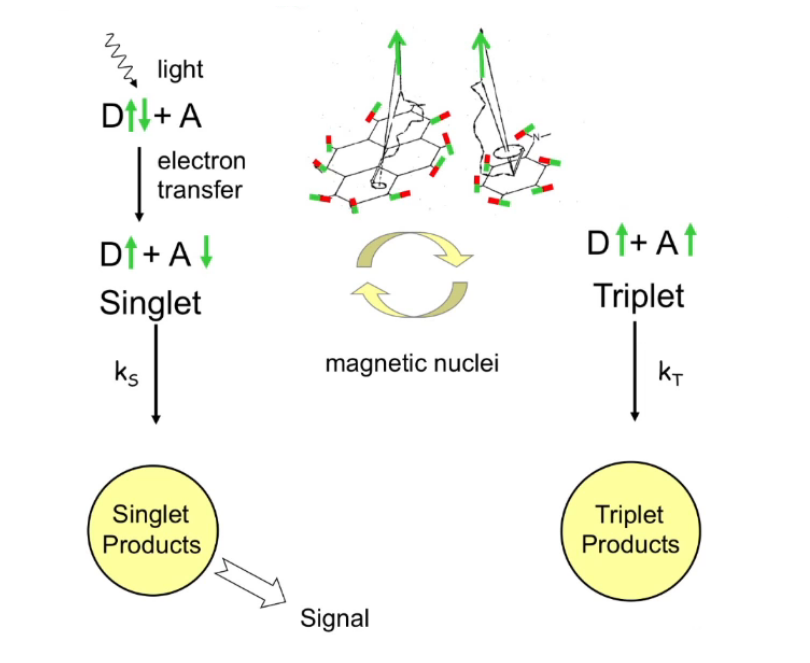
\includegraphics[width=0.7\textwidth]{diagrama}
	\caption{Diagrama del proceso radical-pair. De la charla de T. Ritz, basado en \cite{schulten1978semiclassical}}
	\label{diagrama}
\end{figure}


Este proceso no pertence solo a los avances teóricos si no que se han podido observar experimentalmente sus implicaciones, como en \cite{maeda2008chemical}.

¿Cómo relacionamos esto con el sentido magnetico? Si los animales, en particular los pajaros, poseen este mecanismo para orientarse, entonces los campos magneticos de alta frecuencia afectaran a la sincronizacion del mecanismo de radical par (si el cmapo es lo suficientemente fuertes y tiene la frecuencia adecuada). 
Además, si realizamos este tipo de experimentos, estos no deberian alterar las particulas de oxido de hierro, con lo que sabremos si el mecanismo de par radical influye directamente sobre los animales. 


\section{Sensores óptimos vía moleculas fotoreceptoras}
\spacing{1.5}
Durante las charlas hablamos sobre la experimentación para conseguir un sensor magnético basado en los avances cuanticos de la manera más optima posible.  

Para ello revisitamos algunos de los estudios que se basan principalmente en el enfoque de los sistemas radical-pair y moléculas fotoreceptoras. En particular, los criptocromos, que son los que han mostrado una posibilidad alta de estar involucrados .Los criptocromos son una clase de fotorreceptores de luz azul de plantas y animales que constituyen una familia de flavoproteínas, pueden encontrarse, por ejemplo, en los ojos de algunos pájaros migratorios.




\begin{figure}
	\centering
	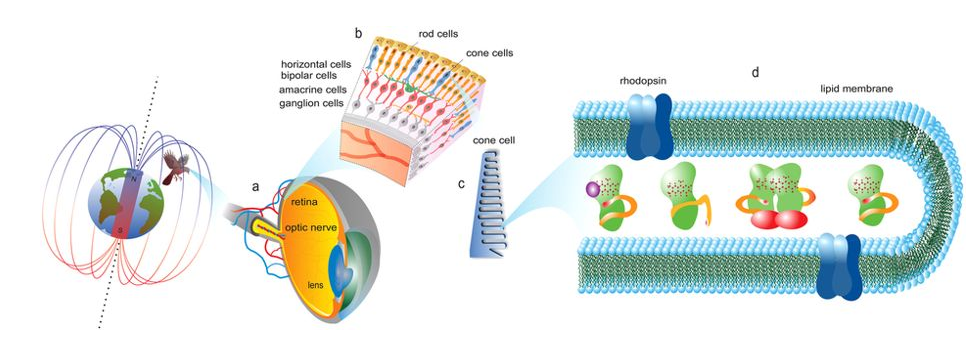
\includegraphics[width=1\textwidth]{ojos}
	\caption{Mecanismo implicado en el sentido magnetico de los pájaros dentro de sus ojos }
	\medskip
	\small
	de \cite{procopio2016inhomogeneous}: \textit{La retina es una capa sensible a la luz en la parte posterior del ojo que convierte las señales de luz, que entran en el ojo de la lente, en señales electroquímicas y transmite estas señales al cerebro a través del nervio óptico. (b) Sección de la retina que muestra los cinco tipos de células dispuestas en capas. La señal primaria se genera en las células del cono del fotorreceptor, pasa a otras capas de células y se transmite al cerebro por las células ganglionares. (c) Disco de los segmentos externos de una célula de cono donde se sugiere que el foto-magnetoreceptor cryptochrome esté localizado15,32. (d) Sección de una membrana de disco de una celda de cono. Las proteínas de rodopsina, representadas en azul, realizan la foto-transducción primaria de información visual. Las proteínas cryptochrome, representadas en verde con el C-terminal en naranja, pueden realizar la transducción primaria de información magnética, a través de la formación de reacciones de pares radicales magnéticamente sensibles. Un conjunto de criptocromos dentro de las células fotorreceptoras puede estar en diferentes estados conformacionales, como (de izquierda a derecha): con el C-terminal en la proximidad del cofactor flavina, con un metabolito unido, en forma dimerizada, con el C-terminal extendido.}

\end{figure}




\section{Notas finales}
\spacing{1.5}


\section*{Referencias}
\bibliographystyle{apalike}
\bibliography{bibliograf}



\end{document}
